\subsection{Sensoren}\label{Sensoren}

\begin{wrapfigure}{R}{0.3\textwidth}
\centering
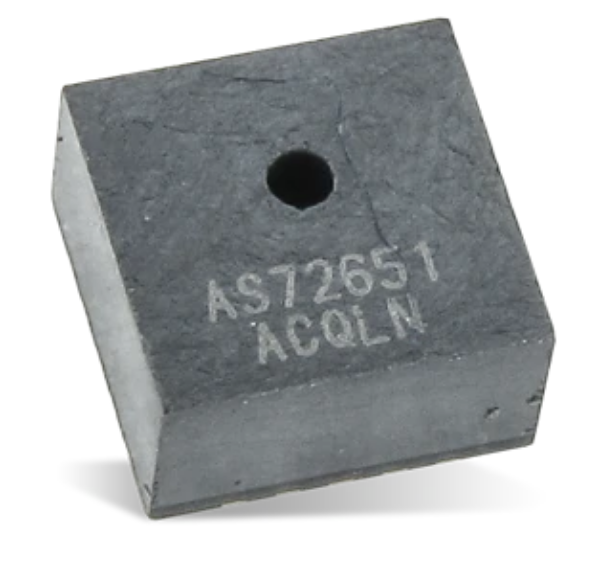
\includegraphics[width=0.25\textwidth]{img/as726X.png}
 \caption{AS726X \cite{Datenblatt_AS7265X}}
\label{fig:AS726X}
\end{wrapfigure}

Die Sensoren aus der AS726X Reihe sind in der Lage Licht, also elektromagnetische Strahlung, zu messen. 
In jedem Sensor sind 6 Photodioden verbaut. 
Vor jeder Photodiode ist ein Silizium-Interferenzfilter montiert, welcher wie ein Bandpassfilter arbeitet. Er ist nur für einen bestimmten Ausschnitt des Lichtspektrums durchlässig.
Jeder Baustein enthält einen Analog-Digital-Wandler mit 16 Bit Auflösung, der den Photostrom aus den Fotodioden integriert. Nach Abschluss einer Messung wird das integrierte Ergebnis in die entsprechenden RAW Data Register übertragen.\\
So kann über das beschriebene Sensorarray die farbliche Zusammensetzung des eingestrahlten Lichts erfasst werden.

\begin{figure}[H]
\centering
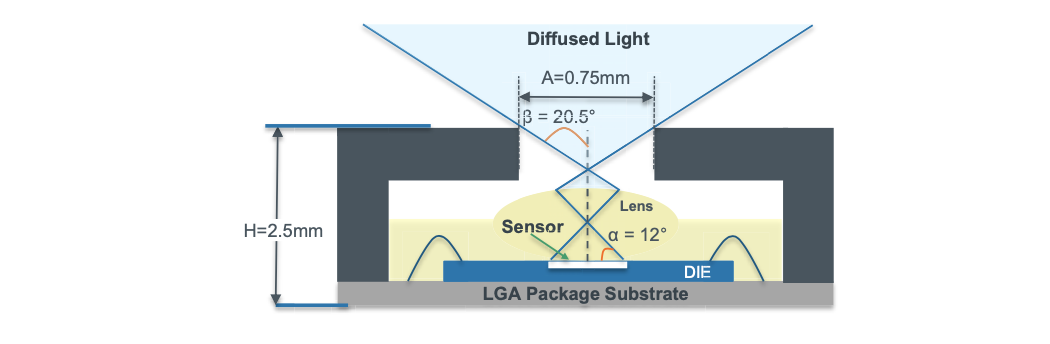
\includegraphics[width=0.9\textwidth]{img/AS726X-seitenansicht.png}
\caption{Seitenasicht AS726X\cite{Datenblatt_AS7265X}}
\label{fig:Seitenasicht-AS726X}
\end{figure}

\noindent Wie in Abbildung \ref{fig:Seitenasicht-AS726X} dargestellt, fällt das Licht durch die Öffnung in der Mitte des Sensors ein. Eine intern verbaute Linse verteilt das Lich auf die Interferenzfilter. Die Genauigkeit der Filter verändert sich je nach Einstrahlwinkel, daher ist es wichtig vor den Sensor noch eine Streuscheibe zu montieren.\\
Die so gemessenen Daten können über UART oder I2C an einen Mikrocontroller übertragen werden. Da über UART nur ein Gerät verbunden werden kann, eignet sich aber für diesen Anwendungsfall nur die I2C Schnittstelle.\\
Alle Sensoren erhalten vom Hersteller dieselbe, nicht veränderbare I2C Adresse: 0x49. Daher muss ein I2C Translator genutzt werden, welcher es ermöglicht mehrere Sensoren im gleichen Bussystem zu adressieren (siehe Abschnitt \ref{I2C-Translator}).\\


\noindent Die Modelle unterscheiden sich durch die verbauten Silizium-Interferenzfilter, also die unterscheidbaren Wellenlängenbereiche sowie in der benötigten Peripherie.
Die grundsätzliche Messmethode ist aber immer gleich.
Im Folgenden werden die verwendeten Sensoren AS7261 (siehe Abschnitt \ref{AS7261}) sowie der AS7265X (siehe Abschnitt \ref{AS7265X}) beschrieben.\\
Intern im Sensor werden aus den RAW-Werten kalibrierte Werte berechnet, jedoch wird keine ausreichende Dokumentation bereitgestellt.
Daher konnte keine konsistente Korrelation zwischen RAW- und kalibrierten Werten ermittelt werden, weshalb sie im Messaufbau nicht verwendet werden.


%\begin{wrapfigure}{L}{0.3\textwidth}
%\centering
%    \caption{Seitenasicht AS726X}
% 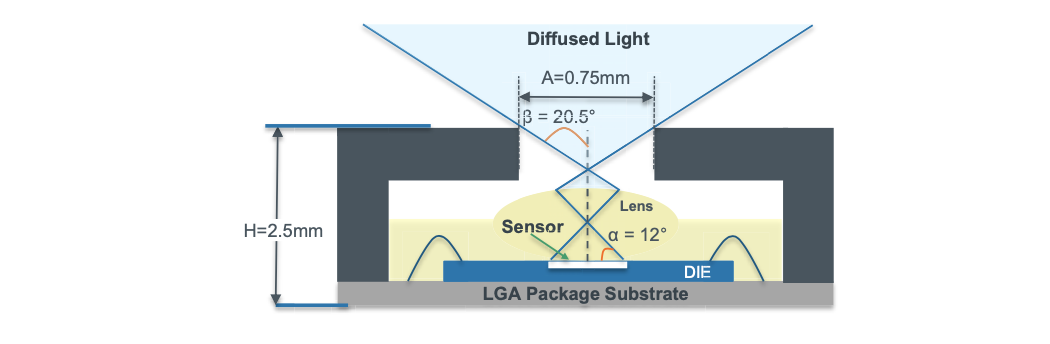
\includegraphics[width=0.7\textwidth]{img/AS726X-seitenansicht.png}
% \caption*{Quelle: Datenblatt AS7261}
%  \label{fig:AS726X}
%\end{wrapfigure}
\newpage
\subsubsection{AS7261}\label{AS7261}
Das Sensorarray des AS7261 unterscheidet zwischen X, Y, Z, Clear, Dark und NIR.
Wobei X, Y und Z nach CIE 1931 definiert sind.
Clear ist eine Fotodiode ohne Filter.
Dark ist eine abgedunkelte Fotodiode und wird nur verwendet um störende Einflüsse zu detektieren.
NIR steht für Near-infrared  (Nah-Infrarot).\\

\begin{figure}[H]
  \centering
 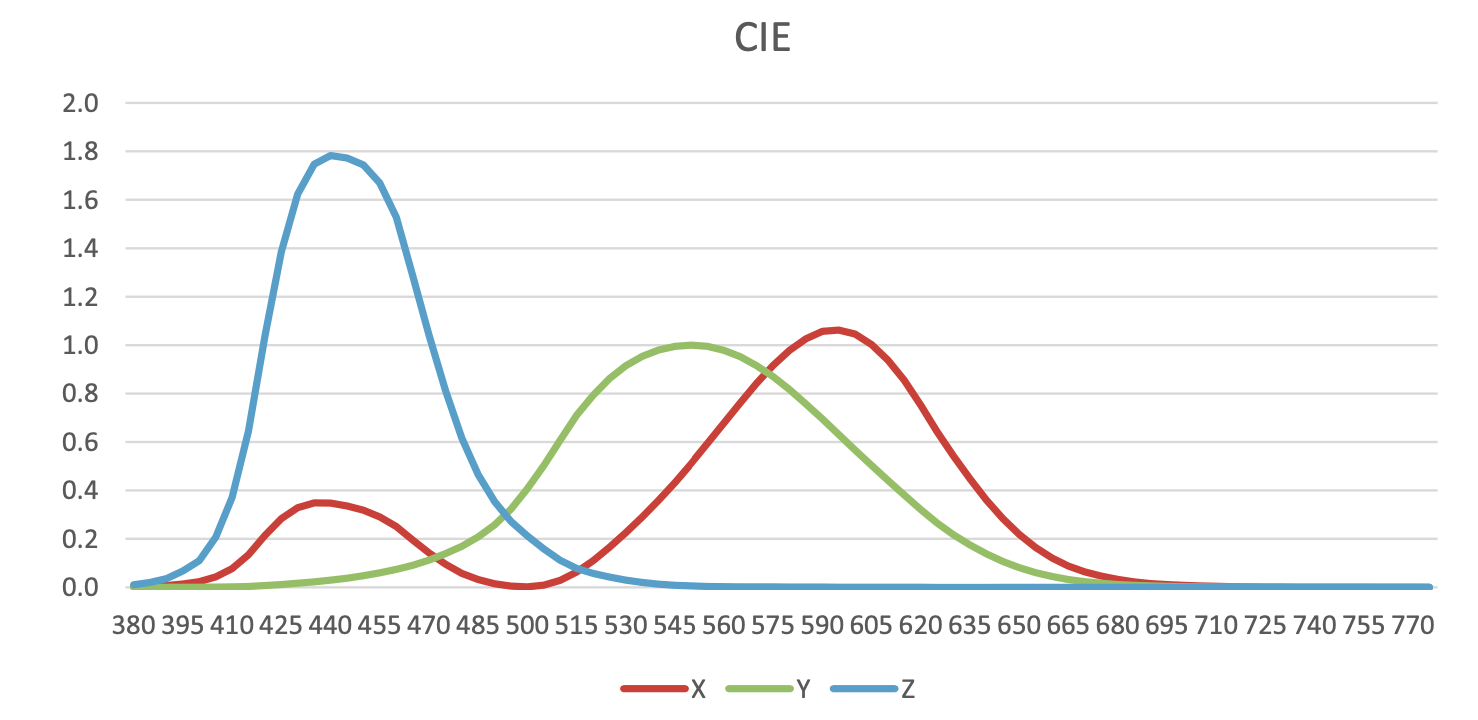
\includegraphics[width=0.6\linewidth]{img/AS7261-Spectral_Responsivity.png}
  \caption{AS7261 Spektrale Empfindlichkeit von X,Y,Z \cite{Datenblatt_AS7261}}
  \label{fig:AS7261-Spectral_Responsivity}
\end{figure}


\begin{wrapfigure}{R}{0.6\textwidth}
\centering
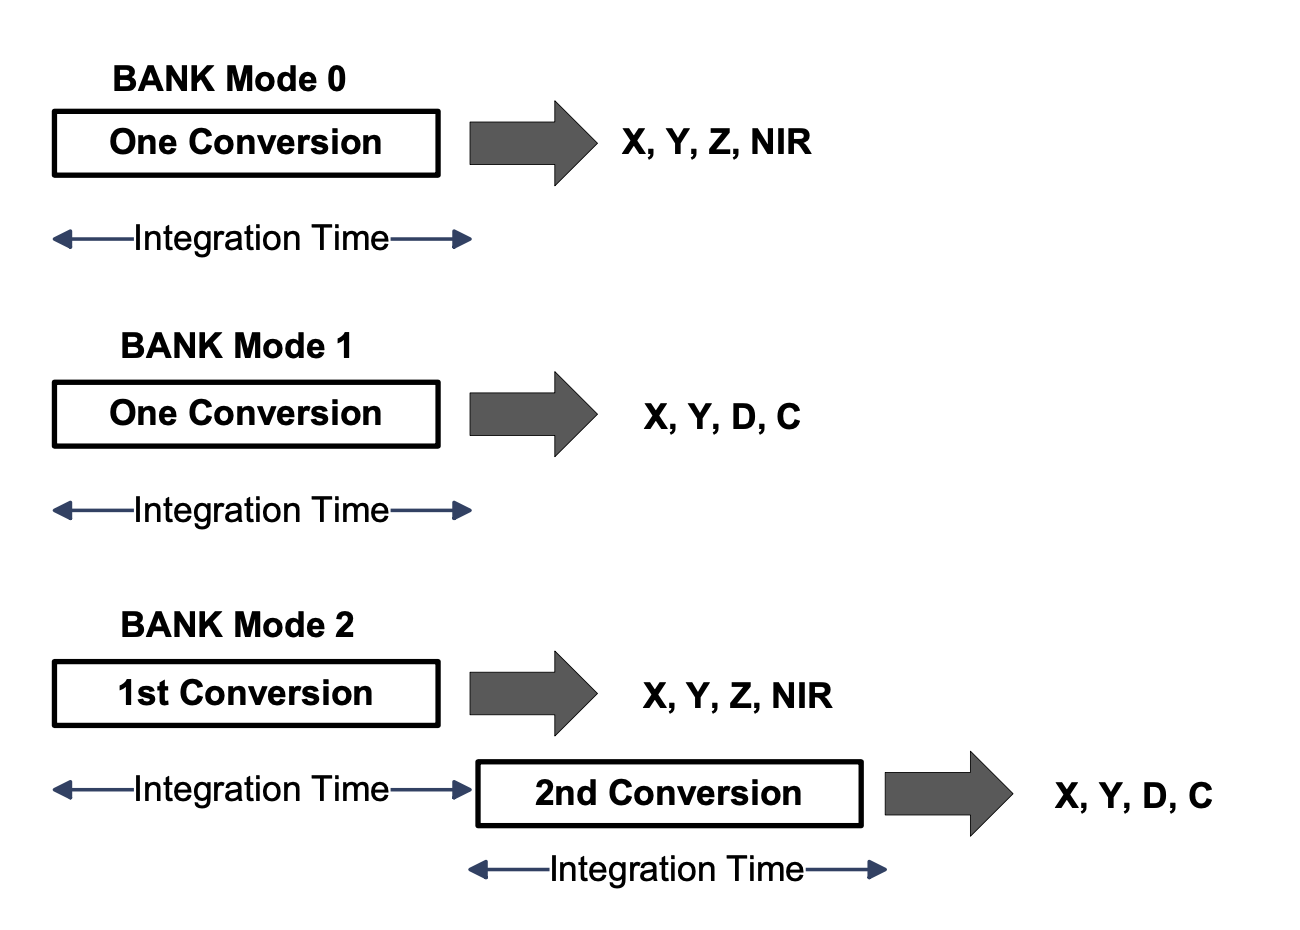
\includegraphics[width=0.5\textwidth]{img/AS7261-Bank_Modes.png}
\label{fig:AS7261-Bank_Modes}
\caption{AS7261-Bank Modes \cite{Datenblatt_AS7261}}
\end{wrapfigure}

\noindent \textbf{Bank Modes:}\\
\label{sec_bank_modes}
Es gibt 3 sogenannte Bank Modes, in denen der Sensor arbeiten kann.\\
\textbf{Bank Mode 0}\\
Die Konvertierungen erfolgen kontinuierlich und Daten sind in den I2C-Registern X, Y, Z und NIR verfügbar.\\
\textbf{Bank Mode 1}\\
Die Konvertierungen erfolgen kontinuierlich und Daten sind in den I2C-Registern X, Y, D und C verfügbar.\\
\textbf{Bank Mode 2}\\
Die Konvertierungen erfolgen kontinuierlich, Daten sind nach zwei Integrationsperioden in den Registern X, Y, Z, NIR, D und C verfügbar. 
In diesem Modus können die kalibrierten, korrigierten Werte auch aus den entsprechenden I2C-Registern abgerufen werden.\\
\textbf{Bank Mode 3}\\
Die Konvertierungen erfolgen nur ein Mal und Daten sind, wie in Bank Mode 2, nach zwei Integrationsperioden in den Registern X, Y, Z, NIR, D und C verfügbar.
Auch die kalibrierten, korrigierten Werte können aus den entsprechenden I2C-Registern abgerufen werden.
Das DATA RDY-Bit wird auf 1 gesetzt, sobald Daten verfügbar sind.\\
Für den hier beschriebenen Messaufbau wird Bankmode 3 verwendet, da so an alle angeschlossenen Sensoren möglichst gleichzeitig eine Messung gestartet werden kann.
Die Daten können nach abgeschlossener Messung an den Raspberry Pi übertragen werden.

\subsubsection{AS7265X}\label{AS7265X}
AS7265X beschreibt AS72651, AS72652 und AS72653 wobei der AS72651 als Master für AS72652 und AS72653 fungiert (Abbildung \ref{fig:S7265X-Scematic}), indem er über einen weiteren separaten I2C Bus ihre Daten abfragt und ansonsten wie der AS7261 arbeitet.
Der angeschlossene Mikrocontroller (Einplatinencomputer) kommuniziert nur mit dem AS72651.

\begin{figure}[H]
  \centering
 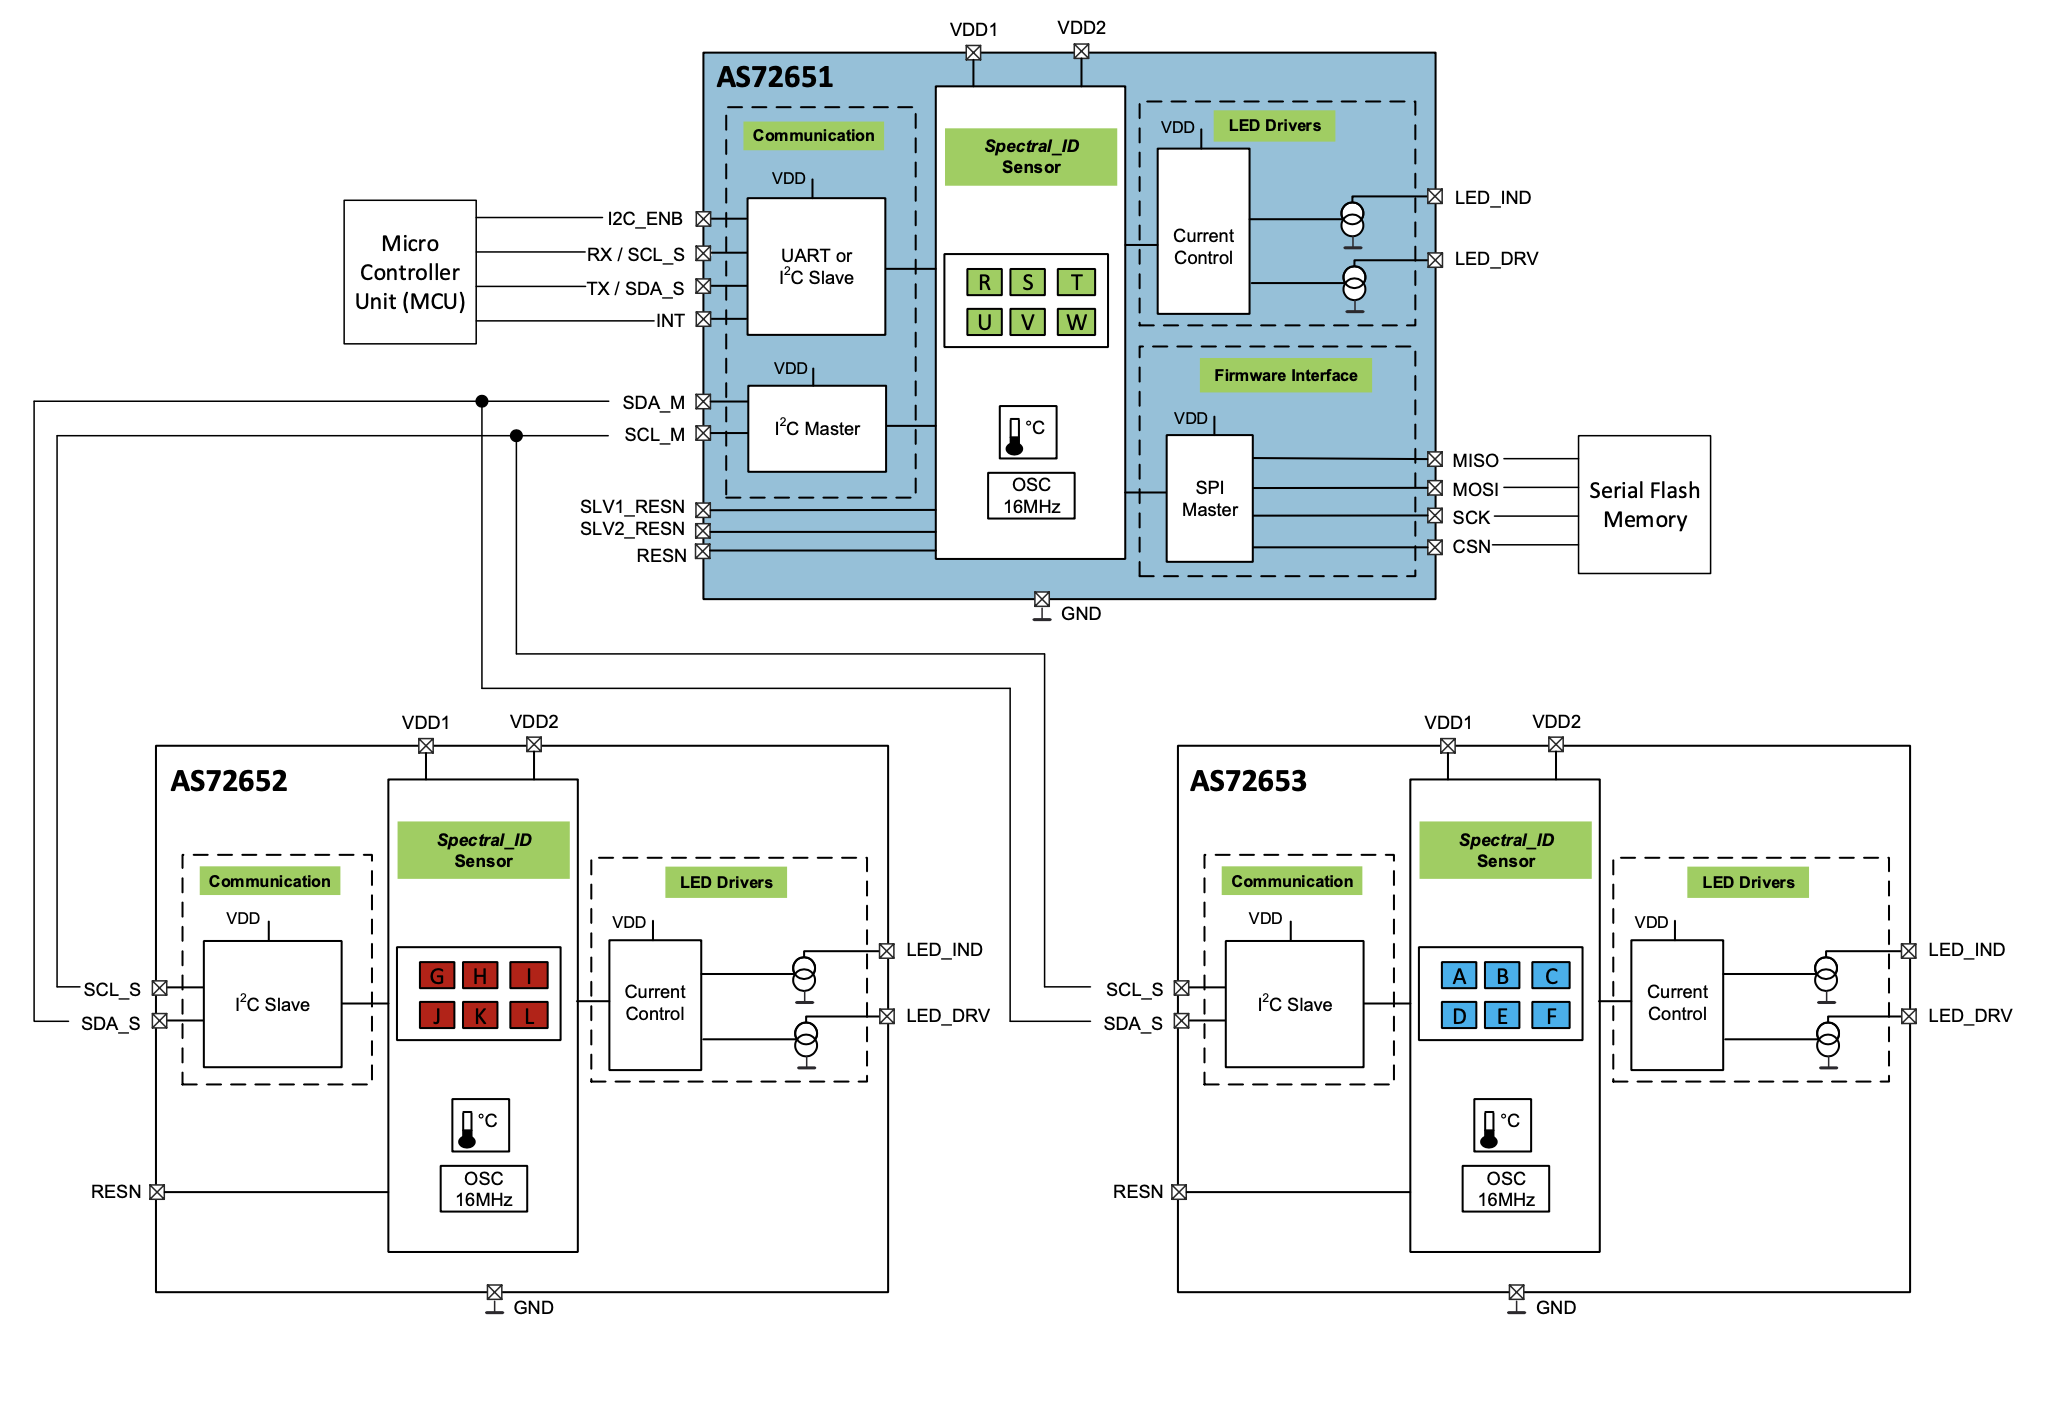
\includegraphics[width=0.9\linewidth]{img/AS7265X-Scematic.png}
 \caption{S7265X-Scematic\cite{Datenblatt_AS7265X}}
  \label{fig:S7265X-Scematic}
\end{figure}


\begin{figure}[H]
  \centering
 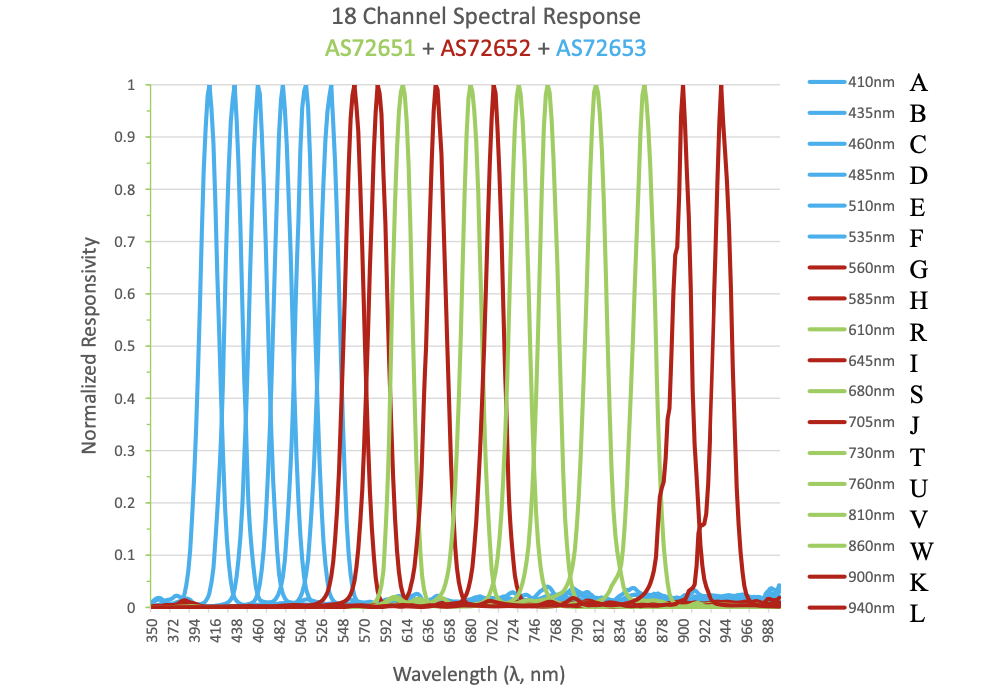
\includegraphics[width=0.9\linewidth]{img/AS7265X-Spectral_Responsivity.png}
 \caption{AS7261-Spectral Responsivity \cite{Datenblatt_AS7265X}}
  \label{fig:AS7261-Spectral_Responsivity}
\end{figure}

\noindent Die drei Sensoren messen in Kombination mit 18  Photodioden mit unterschiedlichen Filtern. So können sie 18 unterschiedliche Frequenz-Channel im Bereich zwischen 410 nm und 940 nm mit einer Halbwertsbreite von jeweils 20 nm erfassen.
Die Frequenz-Channel sind, wie in Abbildung \ref{fig:AS7261-Spectral_Responsivity} zu sehen, mit den Buchstaben A-L gekennzeichnet.\\
Wie der AS7261 kann der AS7265X in 3 Bankmodi betrieben werden, wobei auch für diesen Sensor der Bankmodus 3 verwendet wird, da alle Farbkanäle in einer manuell ausgelösten Messung aufgezeichnet werden sollen.
\newpage
\subsection{Mikrocontroller}\label{Mikrocontroller}
Bei der Auswahl des Mikrocontrollers ist die kleine Bauform, ausreichend langlebiger Speicher sowie eine Netzwerkschnittstelle und I2C Anschluss entscheidend.\\
Die Abfrage der Messdaten sowie die Messkonfiguration soll über einen Fernzugriff möglich sein. Die Daten sollen grafisch in einem Webinterface dargestellt werden, ohne dass eine weitere Serverinstanz benötigt wird. Daher eignet sich ein Linux-Fähiger Einplatinencomputer besser als ein simplerer Mikrocontroller.
Außerdem ermöglicht ein Einplatinencomputer einfache nachträgliche Änderungen, ohne dass eine komplexe Entwicklungsumgebung eingerichtet werden muss.\\

Der Raspberry Pi 4 Model B erfüllt alle diese Anforderungen:

\begin{center}
\begin{tabular}{ c c }
 Abmessungen & 85.6 mm × 56.5 mm \\ 
 Speicher & eMMC Flash Module Socket \\  
 Anschlüsse & Gigabit Ethernet, USB, WLAN \\  
 GPIO & UART, I2C, IO \\  
 RAM & 2 GB \\  
 CPU & Broadcom BCM2711 ARM Cortex A72 \\  
 Preis & 37€ (+20€ für Netzteil und 32GB SD-Karte)  
\end{tabular}
\end{center}
\begin{figure}[H]
  \centering
 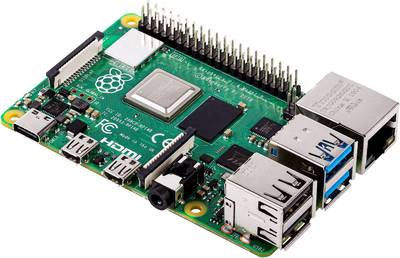
\includegraphics[width=0.5\linewidth]{img/Raspberry-Pi-4-Model-B}
	\caption{Raspberry Pi 4 Model B \cite{raspberrypi_fundation}}
  \label{fig:Raspberry_Pi_4_Model_B}
\end{figure}
An den SD-Kartenslot kann bis zu 256 GB Flash-Speicher angeschlossen werden.
Ein Sensorboard erzeugt etwa 0,73 MB Daten pro Tag.
Bei 12 Sensorboards ist eine noch höhere Effizienz der Datenkomprimierung zu erwarten. Wenn trotzdem 8,78 MB pro Tag angenommen werden, benötigt der Messaufbau maximal 3,3 GB pro Jahr.
Das Betriebssystem, inklusive aller verwendeten Systemkomponenten, benötigt 3,9 GB.
Im Messaufbau werden 32GB SD-Karten verwendet.\\
Die Internetverbindung kann über WLAN oder Ethernet hergestellt werden.
Da eine kabelgebundene Lösung mehr Zuverlässigkeit bietet, wird eine Netzwerkverbindung über Ethernet einer WLAN-Schnittstelle vorgezogen.\\
Die GPIO des Raspebrry Pi arbeiten mit 3,3V.
Der 3,3V Pin des Raspebrry Pi stellt nur 850mA am 3,3V Output bereit.
Da jedes Sensorboard etwa 170 mA benötigt, reichen 850 mA nicht für die maximale Anforderung von 10 Boards aus.
Der 5V-Pin ist direkt mit dem Netzteil verbunden und kann daher genauso viel Leistung wie das Netzteil liefern. Mithilfe eines Abwärtswandlers ist es möglich, die Sensorplatinen mit 3,3V zu betreiben.\\
Die CPU ist für den Anwendungsfall weitaus ausreichend dimensioniert.
In Abbildung \ref{fig:CPU-Performance} ist ein Performancetest zu sehen Die Reihen 1-4 beschreiben die prozentuale CPU Auslastung der jeweiligen Prozessorkerne.
MEM beschreibt die Auslastung des Arbeitsspeichers.\\
Für den Performancetest wurde eine Messung an 4 Sensor Boards mit minimalem Messintervall gestartet.
Außerdem wurden gleichzeitig Daten über Grafana exportiert.\\
\begin{figure}[H]
  \centering
  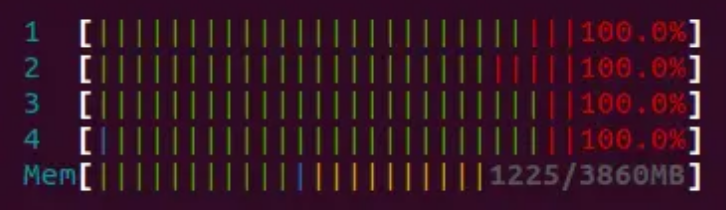
\includegraphics[width=0.7\linewidth]{img/CPU-Performance.png}
  \caption{Screenshot: CPU-Performance}
  \label{fig:CPU-Performance}
\end{figure}
\noindent Der prozentuale Lastdurchschnitt über die letzten 5 Minuten während des Tests wird mit 0,89\% angegeben.

\subsection{I2C Address Translator LTC4316}\label{I2C-Translator}
Da wie in Abschnitt \ref{Sensoren} genannt, alle Sensoren unter derselben I2C Addresse erreichbar sind, wird ein I2C Translator genutzt, um für eine individuelle Adressierung zu sorgen.\\

\begin{figure}[H]
  \centering
 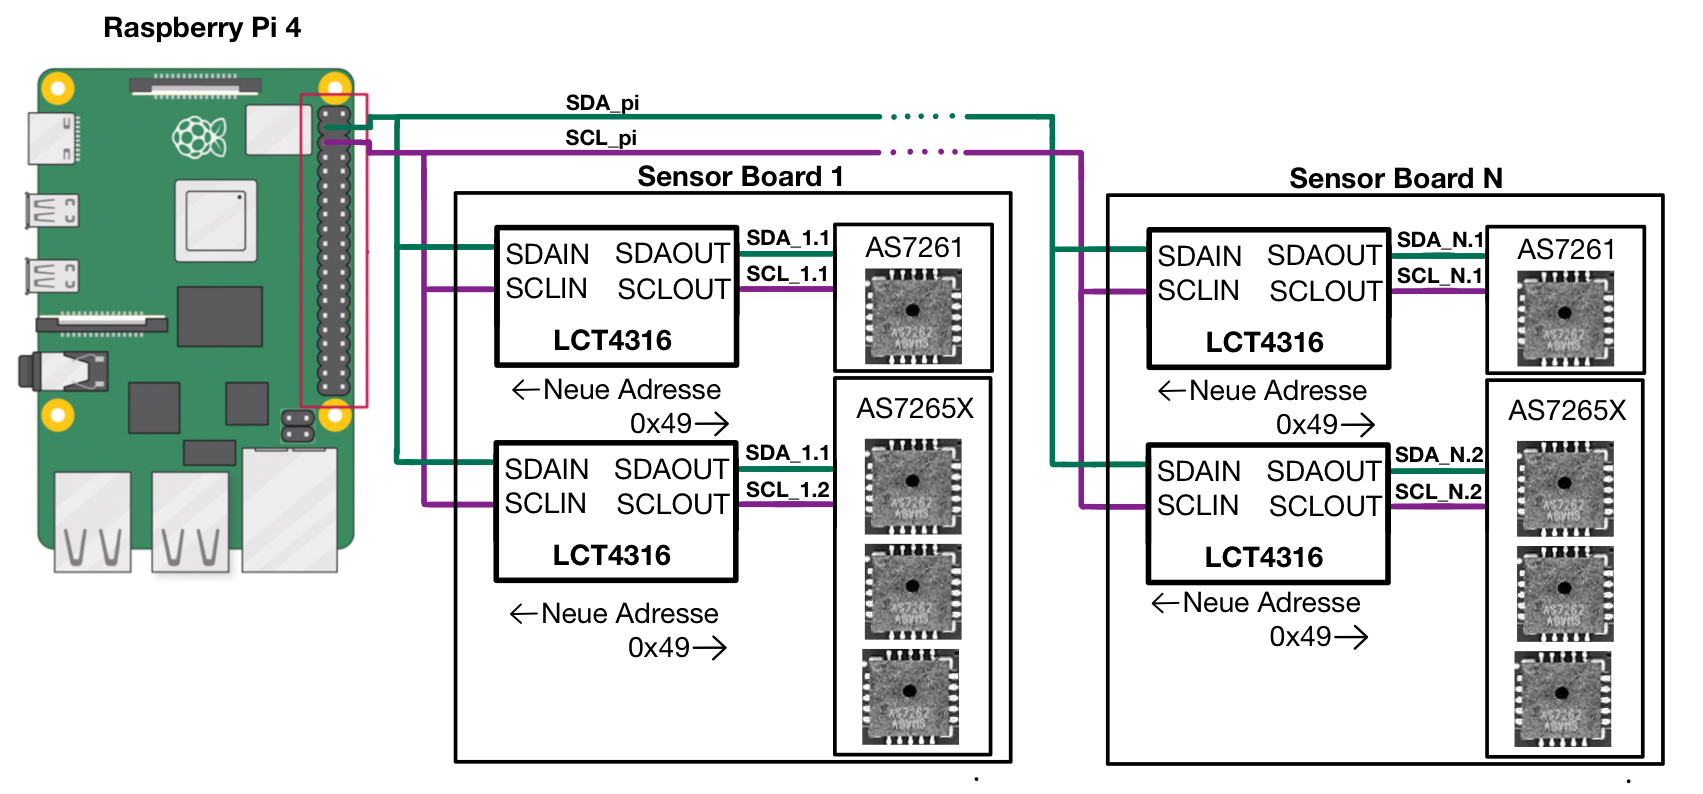
\includegraphics[width=1\linewidth]{img/Adress-Translation}
  \caption{I2C-Bus im Messaufbau \cite{raspberrypi_fundation}}
    \label{fig:adress-translation}
\end{figure}

\noindent Wie in Abbildung \ref{fig:adress-translation} zu sehen, wird für jeden Sensor ein LTC4316 an die Busschnittstelle des Raspberry Pi angeschlossen (SDAIN, SCLIN).\\ 
An jeden LTC4316 wird ein AS7261 oder AS72651 angeschlossen (SDAOUT, SCLOUT).
Bei Kommunikation vom Raspberry Pi zum Sensor wird dann die I2C Adresse mit einem Faktor (Translation Byte), welcher mit diskreten Widerständen eingestellt wird, mit Fomel (\ref{I2C-translation}) verrechnet, um so die Adresse anzupassen (XORH,XORL).
Um das Translation Byte einzustellen, müssen die Widerstände $R_{HT}$, $R_{LT}$, $R_{HB}$ und $R_{LB}$ wie in Abbildung \ref{fig:Translation-Byte} am LTC4316 angeschlossen werden.


\begin{equation} 
\label{I2C-translation}
Sensor Adresse\oplus TranslationByte = NeueAdresse \footnote{xor = $\oplus$}
\end{equation}


\begin{wrapfigure}{R}{0.6\textwidth}
\centering
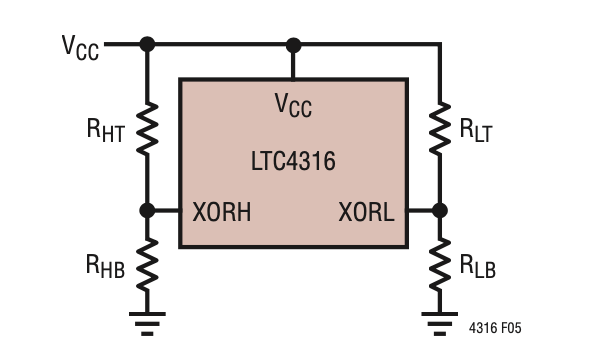
\includegraphics[width=0.6\textwidth]{img/Translation-Byte}
\caption{Translation Byte\cite{Datenblatt_LTC4316}}
\label{fig:Translation-Byte}
\end{wrapfigure}
\bigskip

Beispiel Rechnung\\
$0x49 \oplus 0x01 = 0x48$\\
$0x49 \oplus 0x02 = 0x4b$\\
$0x49 \oplus 0x05 = 0x4c$\\
$0x49 \oplus 0x06 = 0x4f$\\
$0x49 \oplus 0x0A = 0x43$\\
$0x49 \oplus 0x49 = 0x00$\\

\newpage

\noindent 
Tabelle \ref{TranslationByte_Lower} enthält die erforderlichen Widerstandswerte für die diskreten Widerstände $R_{LT}$ und $R_{LB}$ und die daraus resultierenden unteren 4 Bits des Translationsbytes.
Tabelle \ref{TranslationByte_Upper} enthält die erforderlichen Widerstandswerte für die diskreten Widerstände $R_{HT}$ und $R_{HB}$ und die daraus resultierenden oberen 4 Bits des Translationsbytes.

\noindent Durch das Anlöten der jeweiligen Wiederstande können alle 128 mögliche Kombinationen für das Translation Byte erreicht werden. (128 Möglichkeiten ergeben sich da Bit a7 immer 0 ist.) 


\noindent Im Handbuch (Abschnitt \ref{liste_Translationbytes}) ist aufgelistet welche, Translation Bytes bereits verwendet werden. Wenn weitere Sensor-Boards angefertigt werden, ist die Liste dort weiter zu pflegen.

\begin{table}[!ht]
\caption{Untere 4 Bit des Translation Byte}
\label{TranslationByte_Lower}
\centering
\begin{tabular}{c|c|c|c|c|c}
 a3 & a2 & a1 & a0 & $R_{LT}$[$k\Omega$] & $R_{LB}$[$k\Omega$]\\
 0 & 0 & 0 & 0 & Open & Short \\ 
 0 & 0 & 0 & 1 & 976 & 102\\ 
 0 & 0 & 1 & 0 & 976 & 182\\
 0 & 0 & 1 & 1 & 1000 & 280\\ 
 0 & 1 & 0 & 0 & 1000 & 392\\ 
 0 & 1 & 0 & 1 & 1000 & 523\\ 
 0 & 1 & 1 & 0 & 1000 & 681\\ 
 0 & 1 & 1 & 1 & 1000 & 887\\
 1 & 0 & 0 & 0 & 887 & 1000 \\ 
 1 & 0 & 0 & 1 & 681 & 1000\\ 
 1 & 0 & 1 & 0 & 523 & 1000\\
 1 & 0 & 1 & 1 & 392 & 1000\\ 
 1 & 1 & 0 & 0 & 280 & 1000\\ 
 1 & 1 & 0 & 1 & 182 & 976 \\ 
 1 & 1 & 1 & 0 & 102 & 976\\ 
 1 & 1 & 1 & 1 & Short & Open\\
\end{tabular}
\end{table}

\begin{table}[H]
\caption{Obere 4 Bit des Translation Byte}
\label{TranslationByte_Upper}
\centering
\begin{tabular}{c|c|c|c|c|c|c}
 a7 & a6 & a5 & a4 & $R_{HT}$[$k\Omega$] & $R_{HB}$[$k\Omega$]\\
 0 & 0 & 0 & 0 & Open & Short \\ 
 0 & 0 & 0 & 1 & 976 & 102\\ 
 0 & 0 & 1 & 0 & 976 & 182\\
 0 & 0 & 1 & 1 & 1000 & 280\\ 
 0 & 1 & 0 & 0 & 1000 & 392\\ 
 0 & 1 & 0 & 1 & 1000 & 523\\ 
 0 & 1 & 1 & 0 & 1000 & 681\\ 
 0 & 1 & 1 & 1 & 1000 & 887\\

\end{tabular}
\end{table}

\subsection{Companion Flash}
\label{sec_Companion_Flash}
Die Sensoren AS7261 und AS72651 benötigen einen Flash-Speicher, von welchem sie ihre Firmware laden können.
Die jeweilige Firmware von AMS wird mithilfe von Flashcat-USB, einem USB Memory Programmer über das SPI (Serial Peripheral Interface), auf den Flash Speicher übertragen.
Ein Leitfaden für diesen Vorgang wird von AMS unter dem Titel ``How to Program AS72xx Firmware with FlashCatUSB'' bereitgestellt und ist im Anhang zu finden.\\
%https://ams.com/documents/20143/36005/AS72xx_AN000488_3-00.pdf/ab1c985f-785f-7431-99d5-ddea807585db
Der AT25SF041-SSHD-B wurde aus der von AMS bereitgestellten Liste kompatibler Flash-Speichern\footnote{AS726x Design Considerations - 2.5 Flash Memory} ausgewählt, da er am günstigsten ist. 
Für den Messaufbau werden folgende Versionen verwendet.

\begin{tabular}{ l|l } 

  Chip  & Firmware \\ 
 \hline
 AS7261  & AS7261\_complete.bin \\ 
 
 AS726X & AS7265\_complete\_moonlight\_v1.bin\\ 

\end{tabular}
\medskip

Die Binary-Files  sind im Anhang zu finden.\\



